\documentclass[12pt,a4paper]{article}

\usepackage{amsmath}
\usepackage{natbib}
\usepackage{graphicx}
\usepackage{subcaption}
\usepackage[margin=0.75in]{geometry}
\usepackage{titlesec}


\begin{document}

\author{Looking at example websites and gathering requirements\vspace{-2ex}}
\date{\vspace{-5ex}}
\title{Reading-Observations\vspace{-2ex}}

\maketitle

\section{Sports Centres}
\subsection{University Sports Centres}

\begin{center}
	\textbf{The Edge:} https://sport.leeds.ac.uk/the-edge/

	\textbf{Beckett Sports Centre:} https://www.leedsbeckett.ac.uk/sport/
\end{center}

\subsubsection{Landing Pages}

\begin{center}
	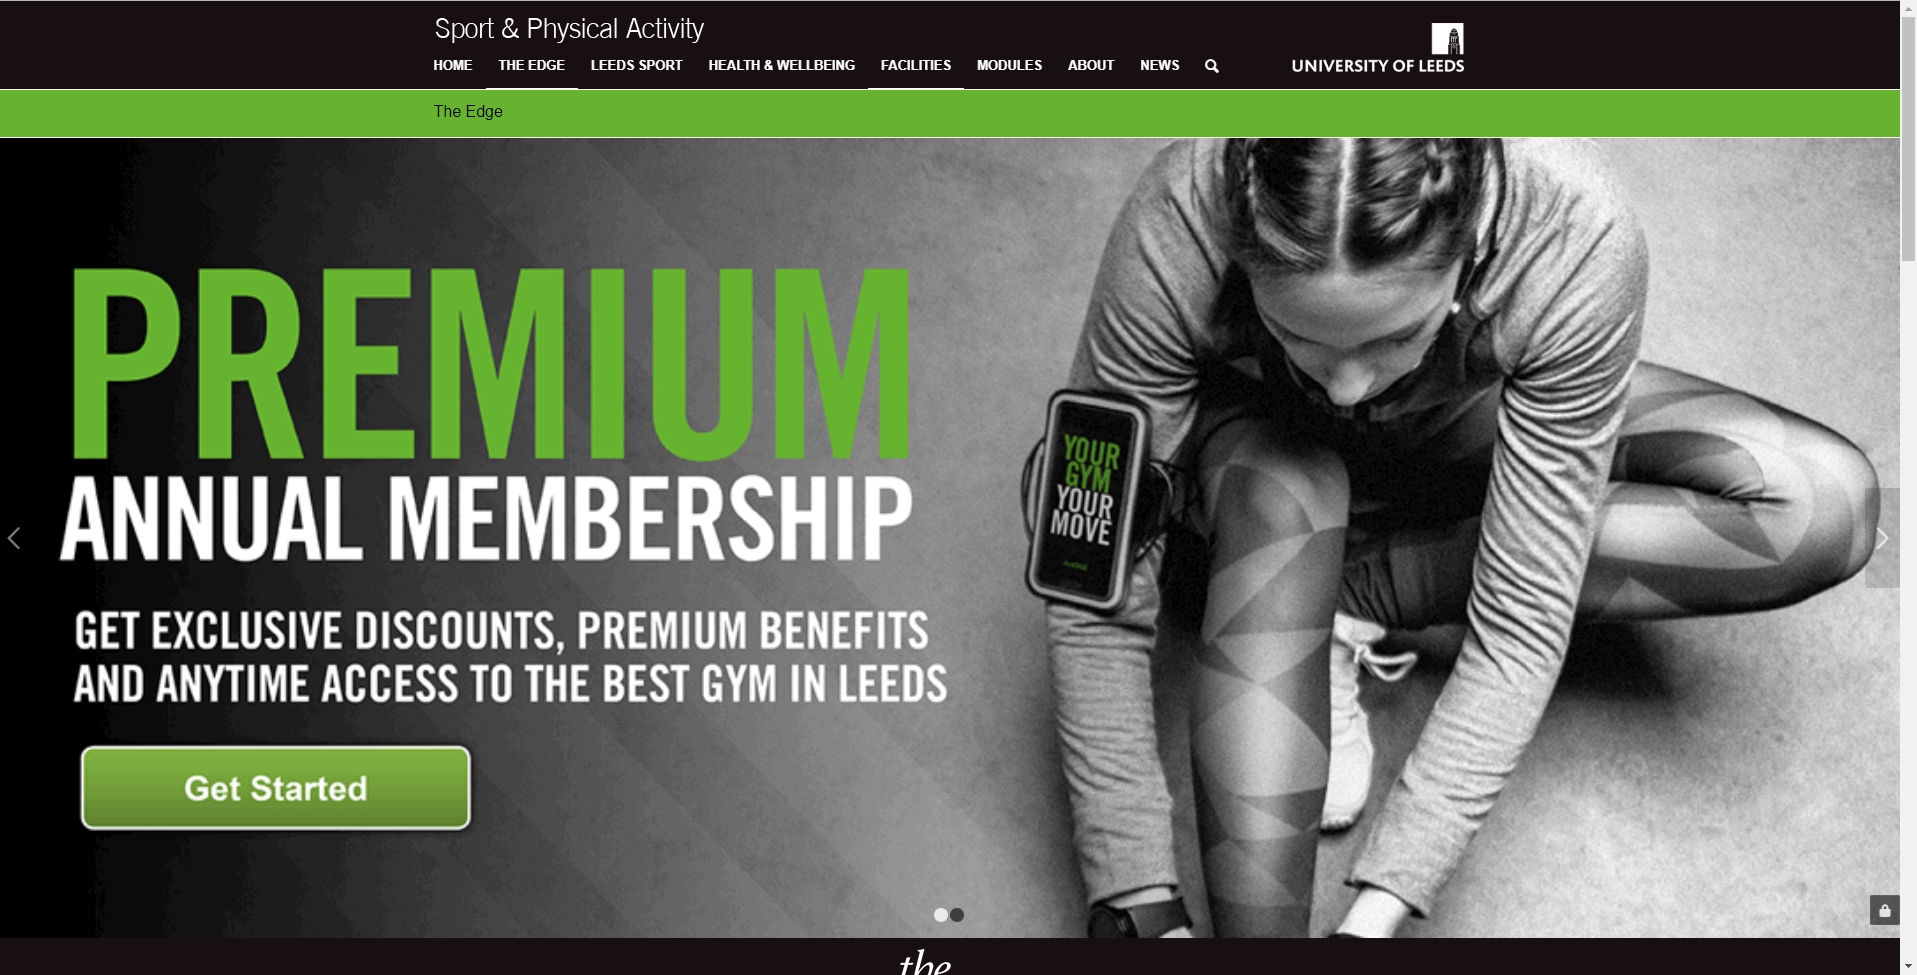
\includegraphics[width=0.7\linewidth]{img/edge-sports-centre.png}\\
	 \textbf{The Edge landing page}
\end{center}

\begin{center}
	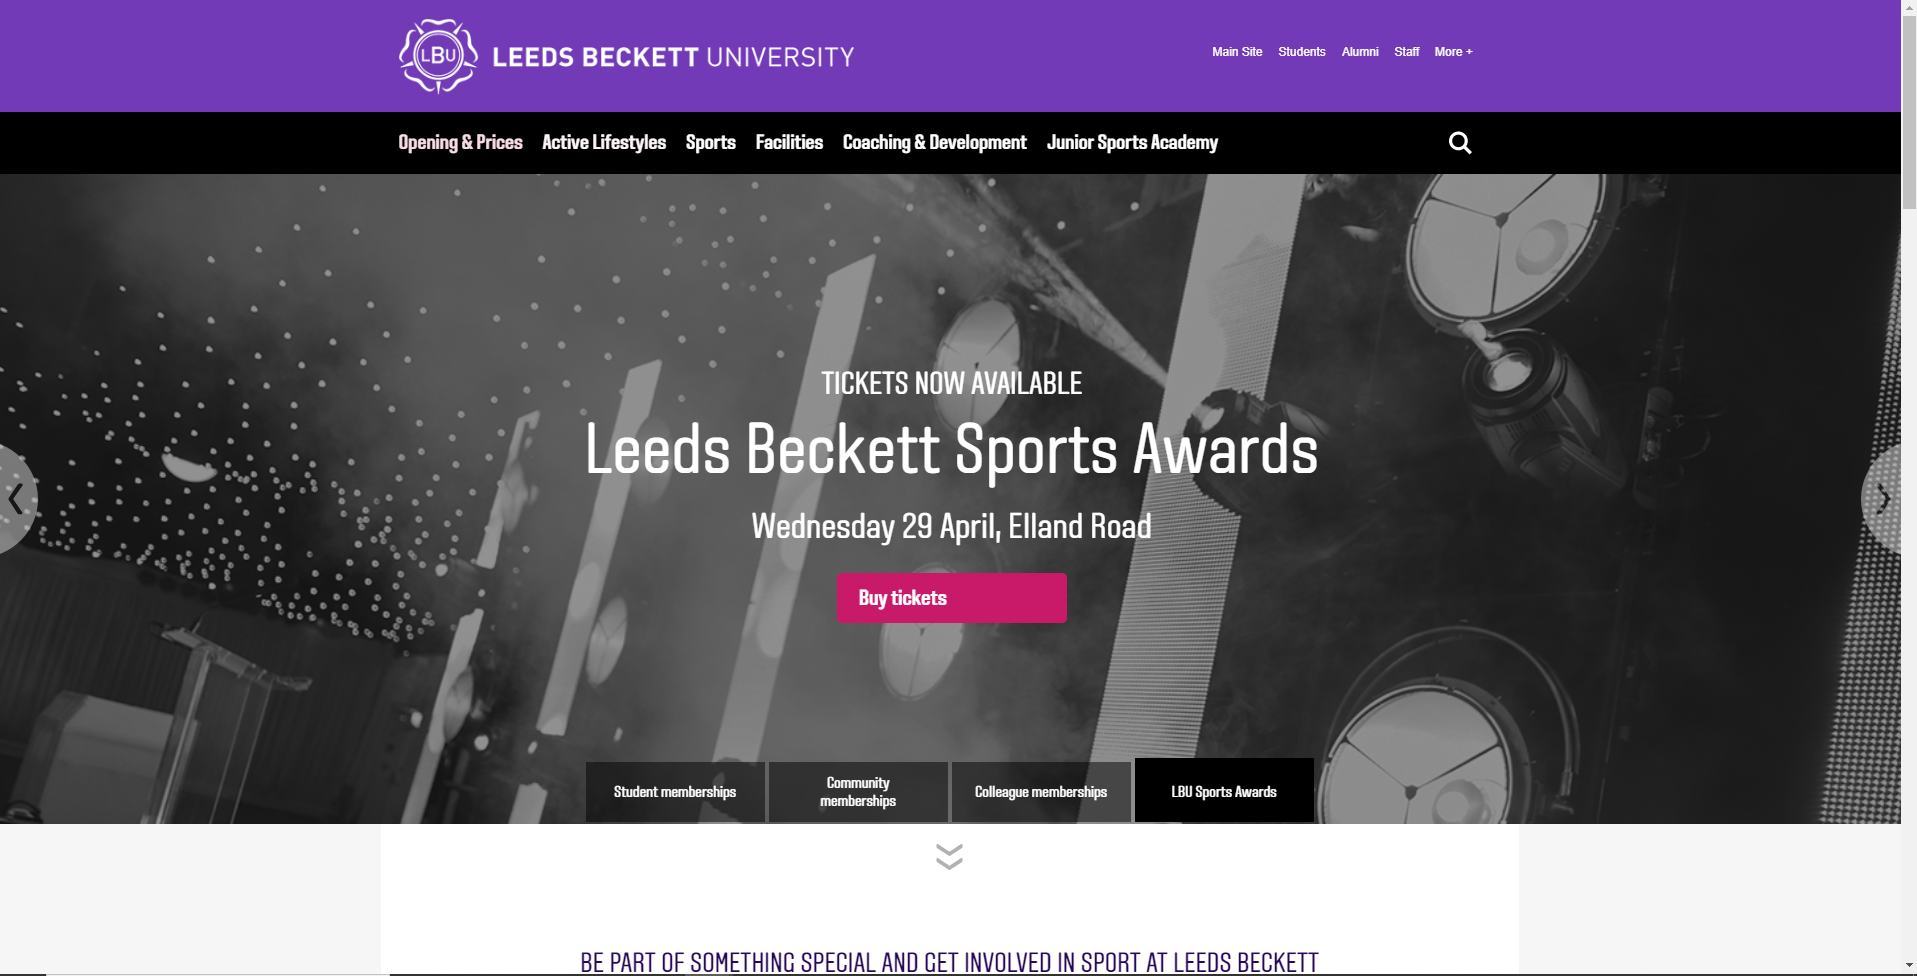
\includegraphics[width=0.7\linewidth]{img/beckett-sports-centre.png}\\
	\textbf{Beckett Sports Centre landing page}
\end{center}




\begin{itemize}
	\item Both have landing pages features large, bold images to grab the users attention
	
	\item The first thing you see on both websites is the membership and pricing options (below jumbotron on beckett)
	
	\item Both have specific section for sports, listing all the sports available in the sports centre
	
	\item Both have specific section to highlight the facilities available - linked to which sports use them 
	
	\item Both have sections to focus on health and well-being and is clearly promoted on both websites
\end{itemize}

\subsubsection{Sports List}
\begin{center}
	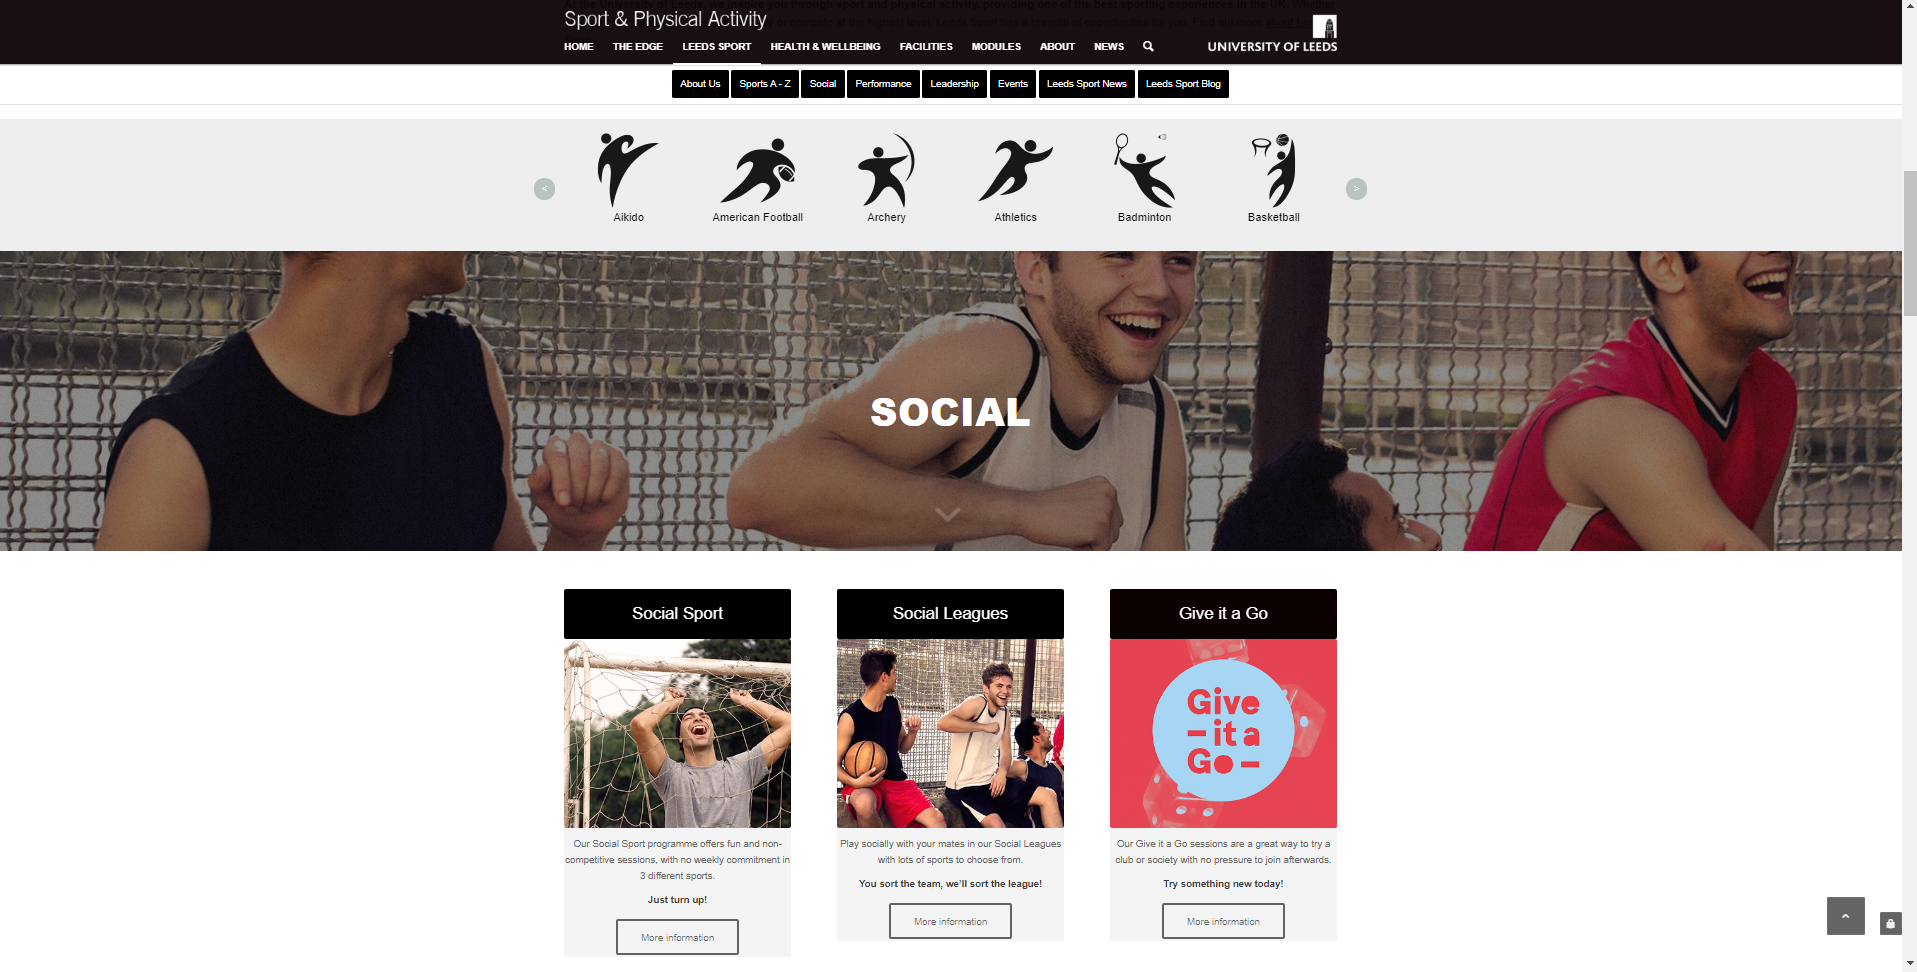
\includegraphics[width=0.7\linewidth]{img/edge-sports-list.png}\\
	 \textbf{The Edge sports list}
\end{center}

\begin{center}
	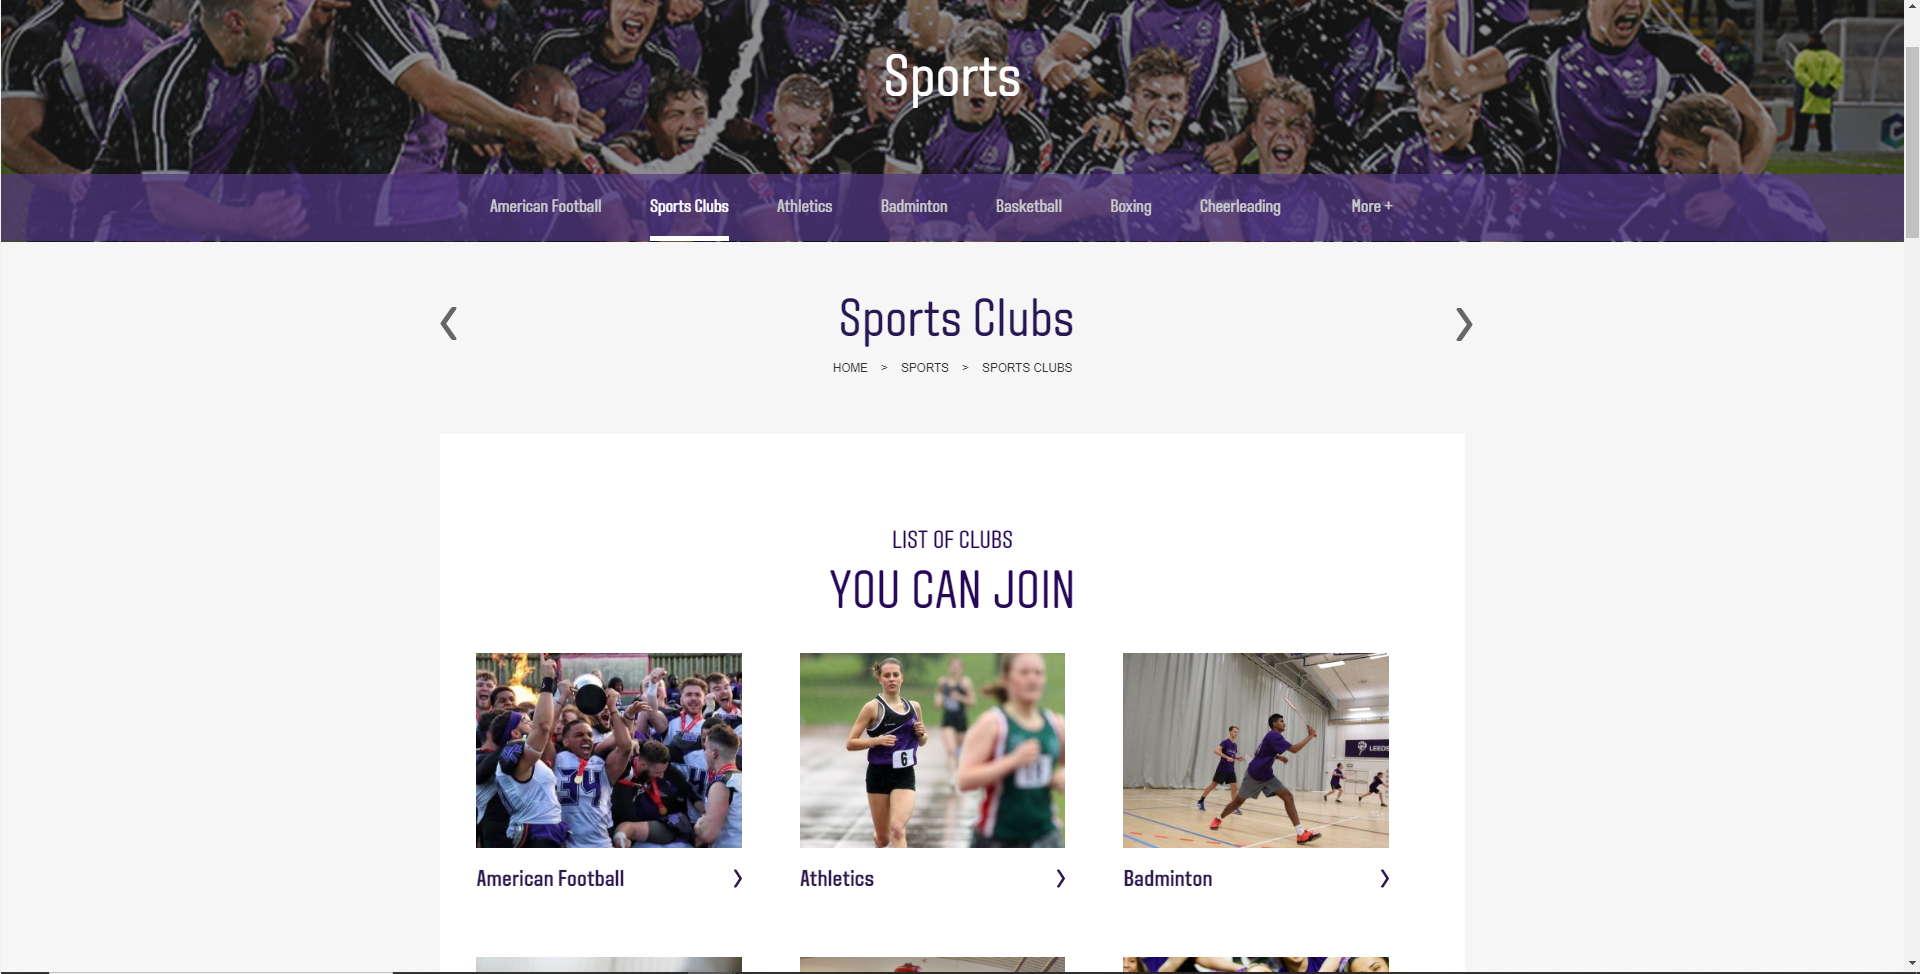
\includegraphics[width=0.7\linewidth]{img/beckett-sports-list.png}\\
	\textbf{Beckett Sports Centre sports list}
\end{center}

\begin{itemize}
	\item Both use a list style with cards displaying the different sports available at the centres; The Edge groups these, whereas Beckett just lists A-Z
	
	\item Both feature images of each of the relative sport, presumably from the centre itself 
	
	\item both use a centre container with the left and right of the page been free; easier for mobile devices
\end{itemize}


\subsection{Leeds City Council Sports Centres}

\begin{center}
	\textbf{Website:} https://active.leeds.gov.uk/findacentre
\end{center}

\subsubsection{Landing Page}

\begin{center}
	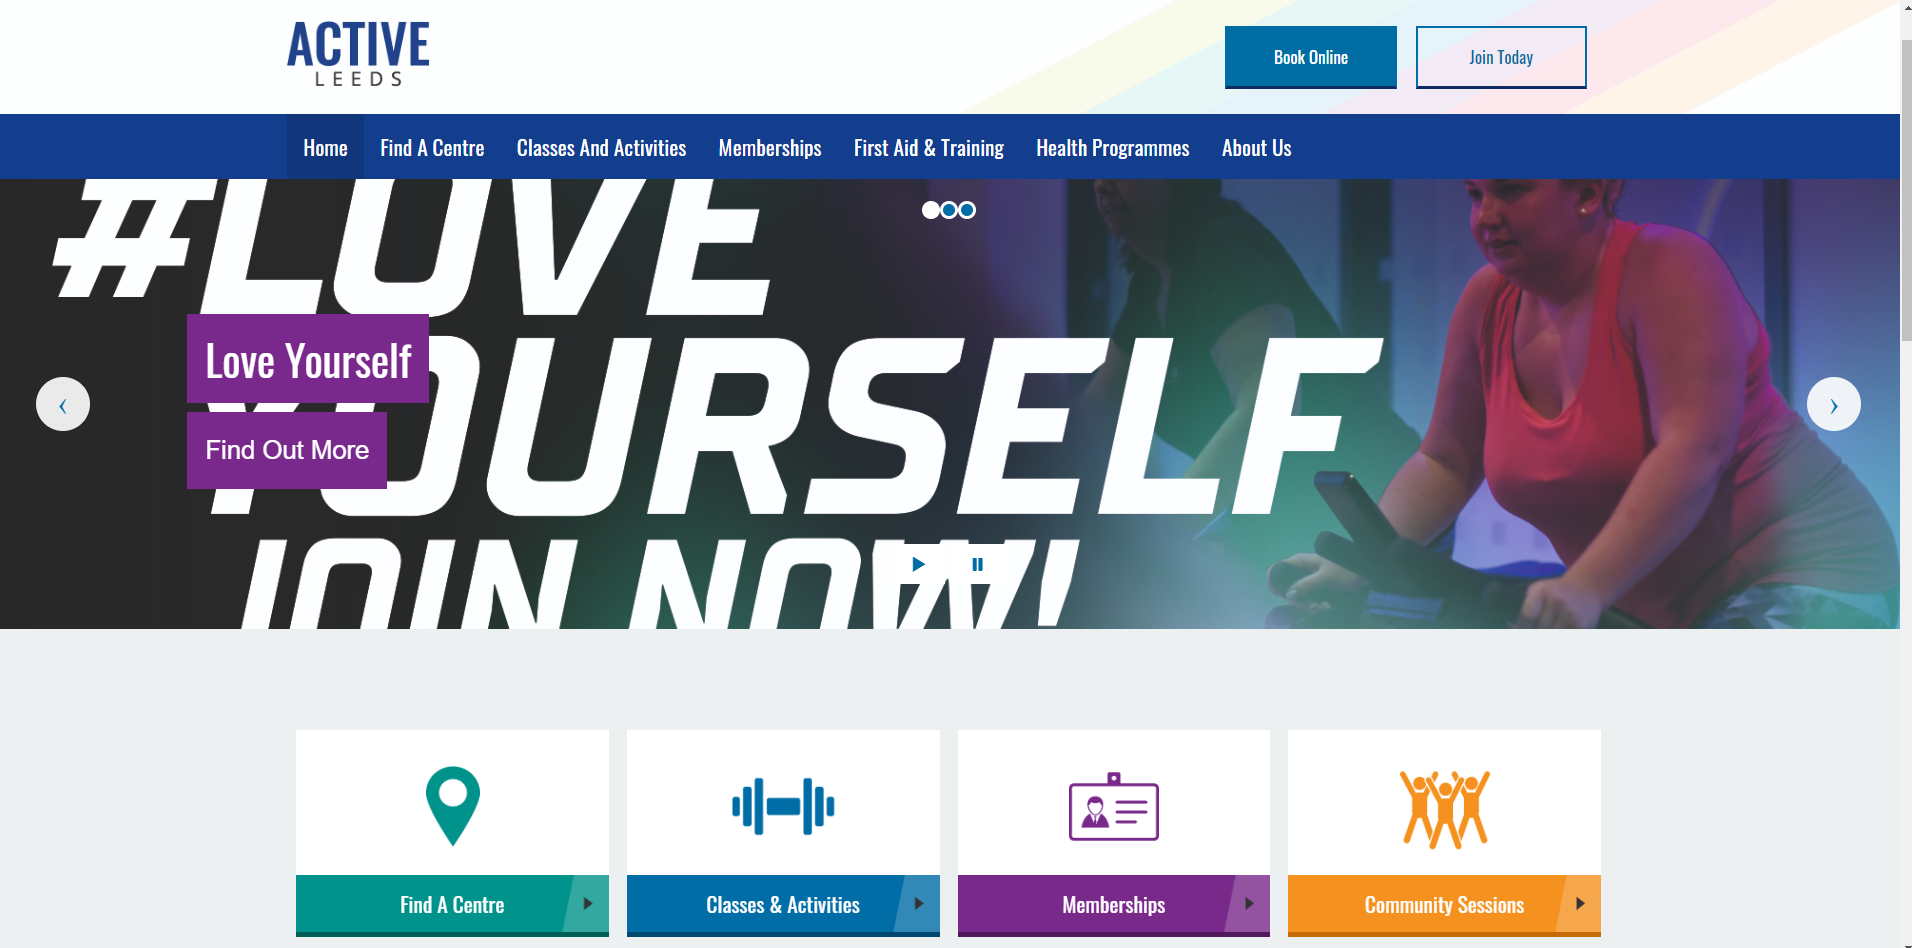
\includegraphics[width=0.7\linewidth]{img/leeds-city-council-sports-centres.png}\\
	\textbf{Active Leeds landing page}
\end{center}

\begin{itemize}
	\item Uses the same large bold images and jumbotron on the landing page to grab attention
	
	\item First thing you see is a health and well-being promotion
	
	\item Since the purpose of the website is to find Leeds City Council Sports Centres, finding a centre, booking sessions and memberships are clearly highlighted on the landing page
	
	\item As with the previous websites, has a specific section to list sports and activities available, including booking these with trainers
\end{itemize}


\subsubsection{Sports List}
\begin{center}
	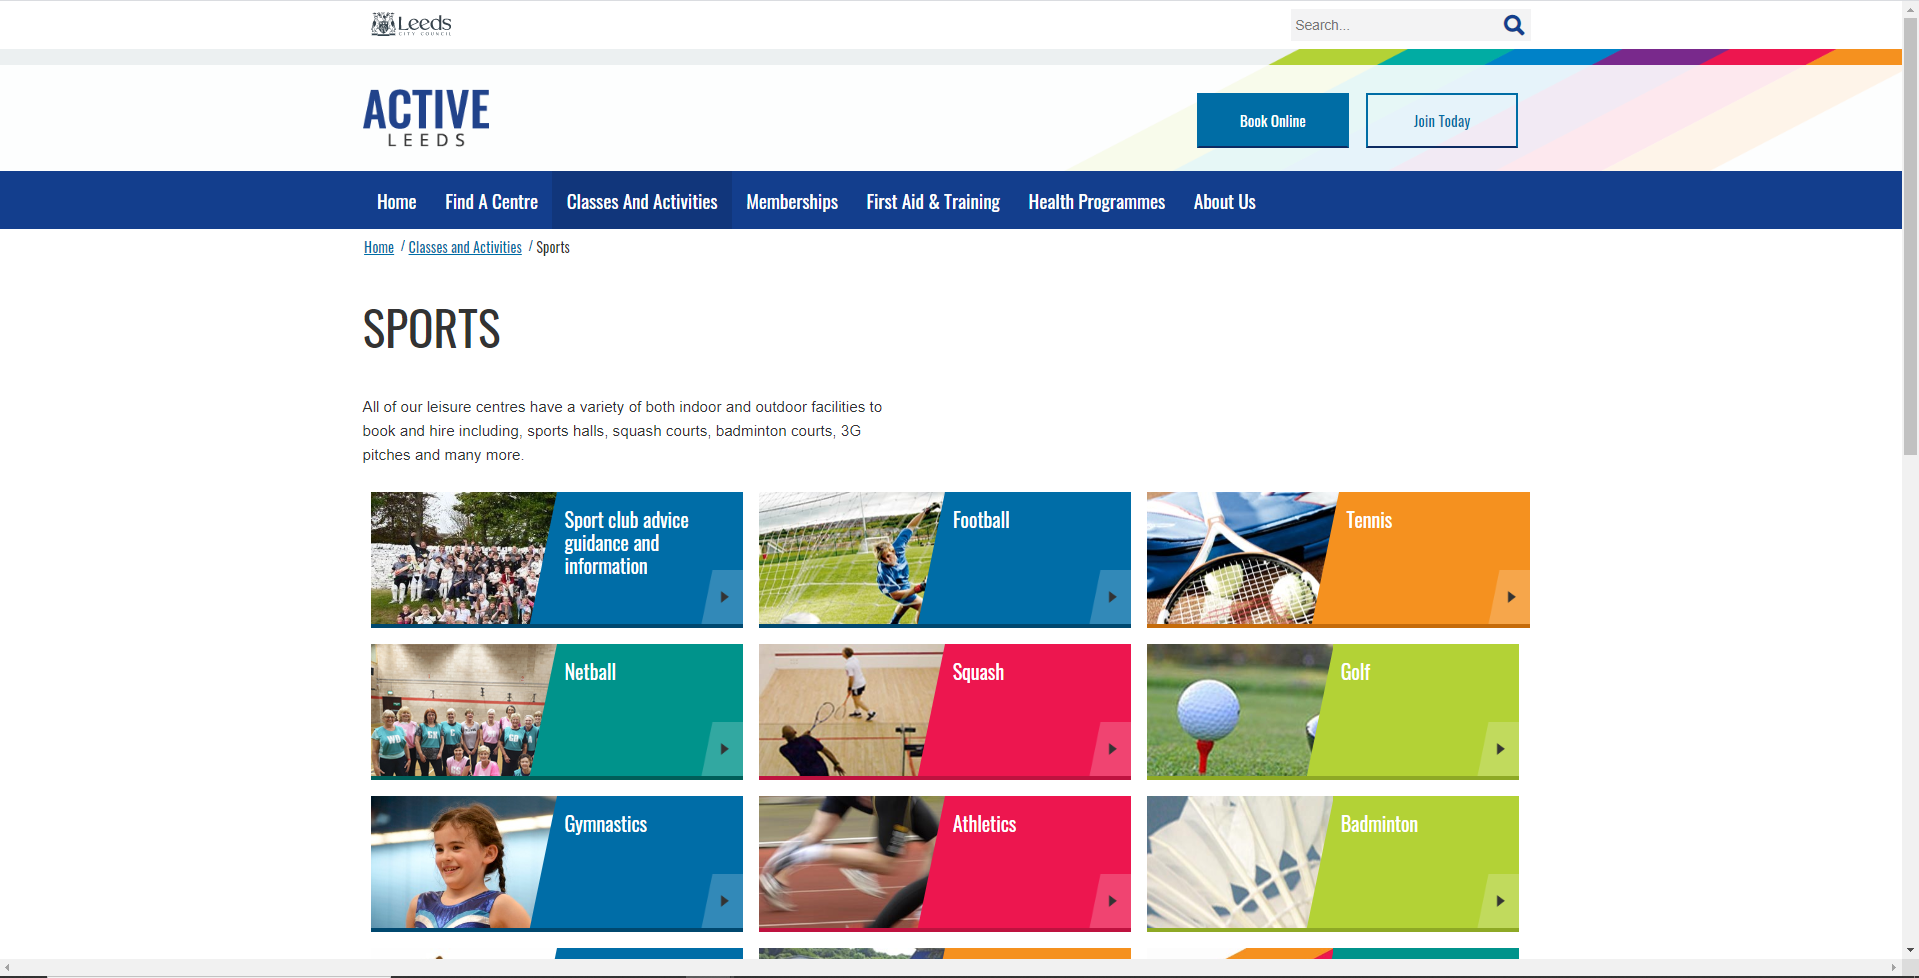
\includegraphics[width=0.7\linewidth]{img/leeds-city-council-sports-list.png}\\
	\textbf{Active Leeds sports list}
\end{center}

\begin{itemize}
	\item Uses the same list-style with cards to display each of the sports  available 
	
	\item Also includes an image relative to each sport 
\end{itemize}


\subsection{Other Notable Websites}

\begin{itemize}
	\item \textbf{Wellsway Sports:} https://www.sportwellsway.com/ - shows good example of landing page with navigation; booking, membership, hire etc.
	
	\item \textbf{Leisure Centre:} https://www.leisurecentre.com/ - shows a good example of a clean, minimalist design employed within a similar site 
\end{itemize}

\section{Gyms}

\begin{center}
	\textbf{Puregym:} https://www.puregym.com/
	
	\textbf{The Gym:} https://www.thegymgroup.com/
	
	\textbf{Exersise4Less:} https://www.xercise4less.co.uk/
	
	\textbf{Firehouse Fitness Gyms:} https://www.firehousefitness.co.uk/
\end{center}

\begin{center}
	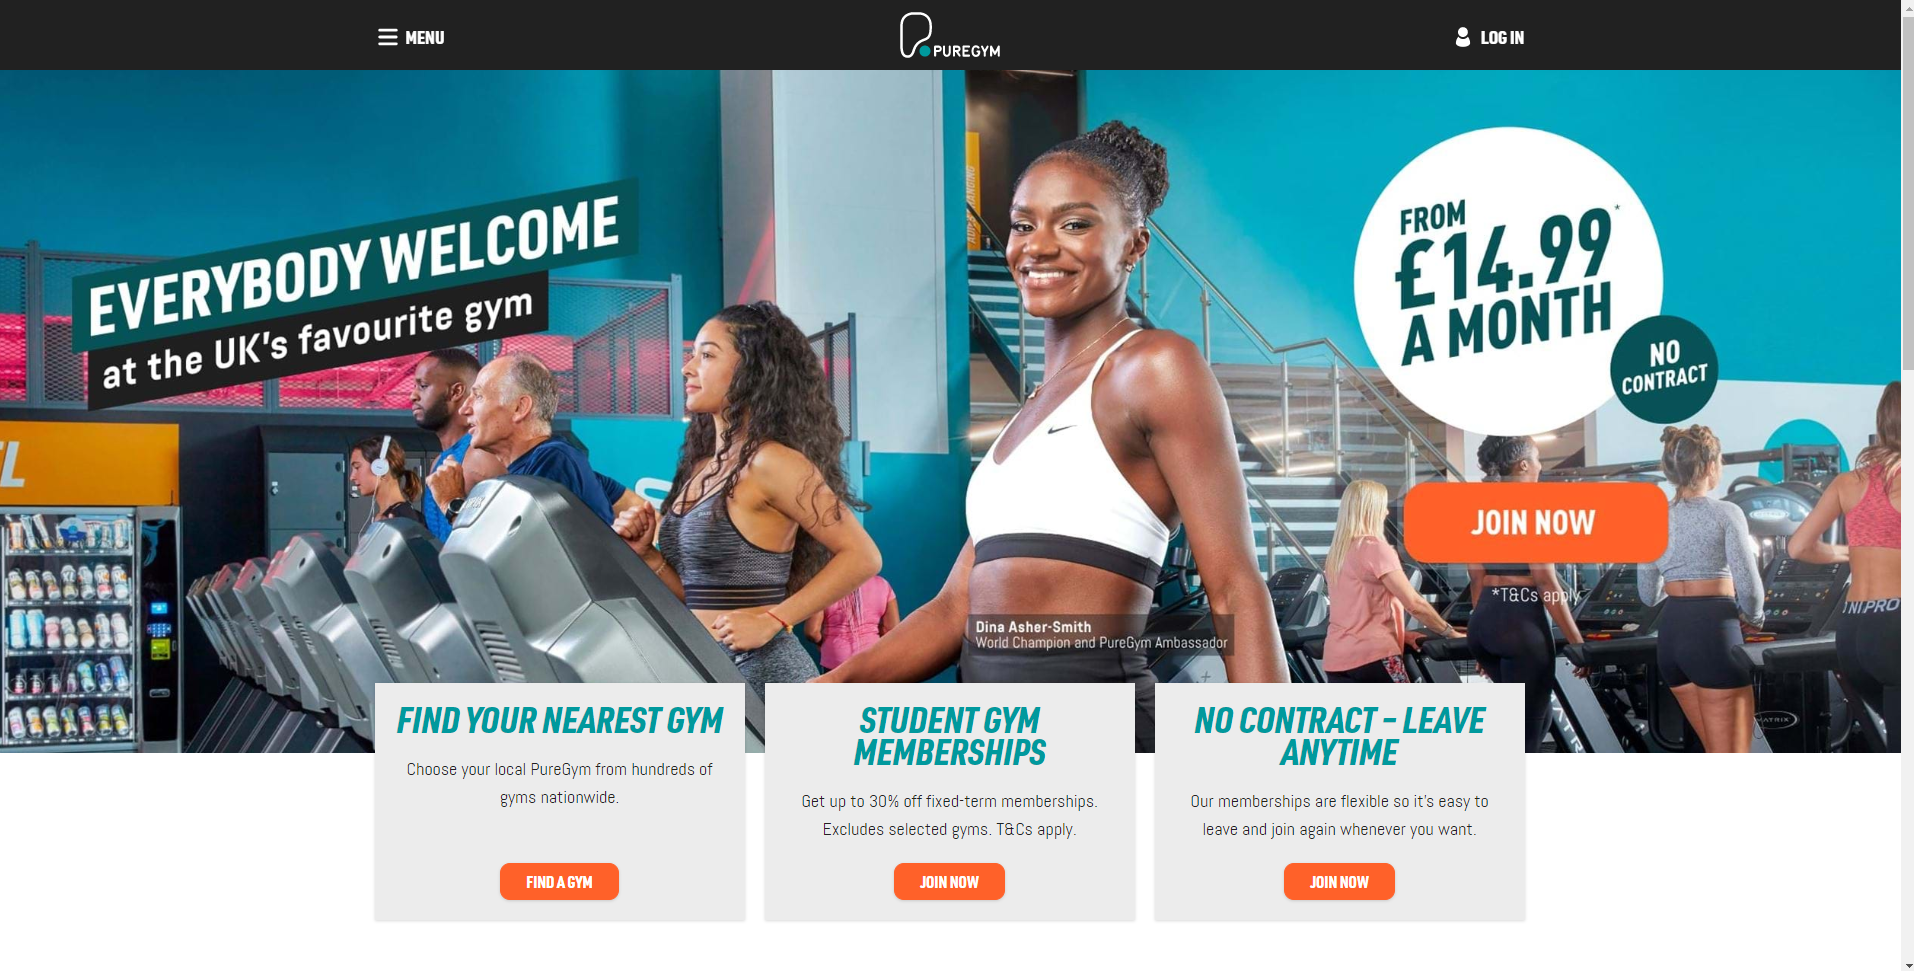
\includegraphics[width=0.7\linewidth]{img/gym/puregym-landing.png}\\
	 \textbf{Puregym landing page}
\end{center}

\begin{center}
	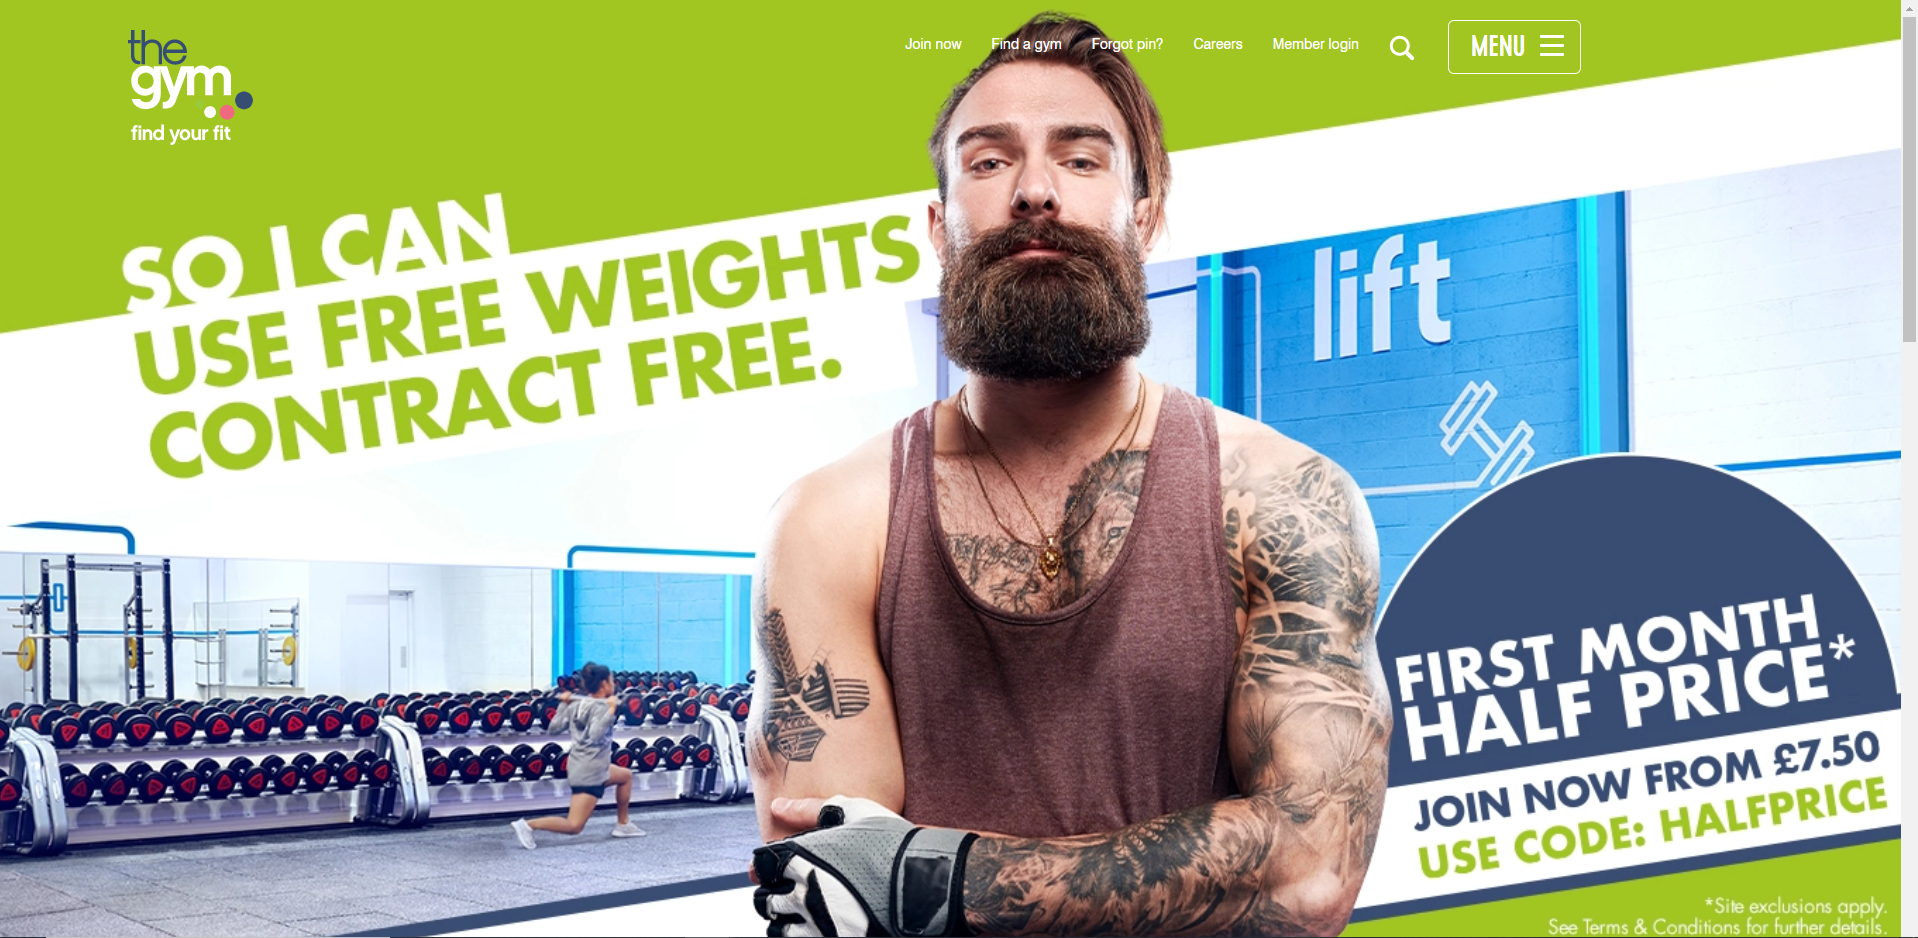
\includegraphics[width=0.7\linewidth]{img/gym/the-gym-landing.png}\\
	\textbf{The Gym landing page}
\end{center}

\begin{center}
	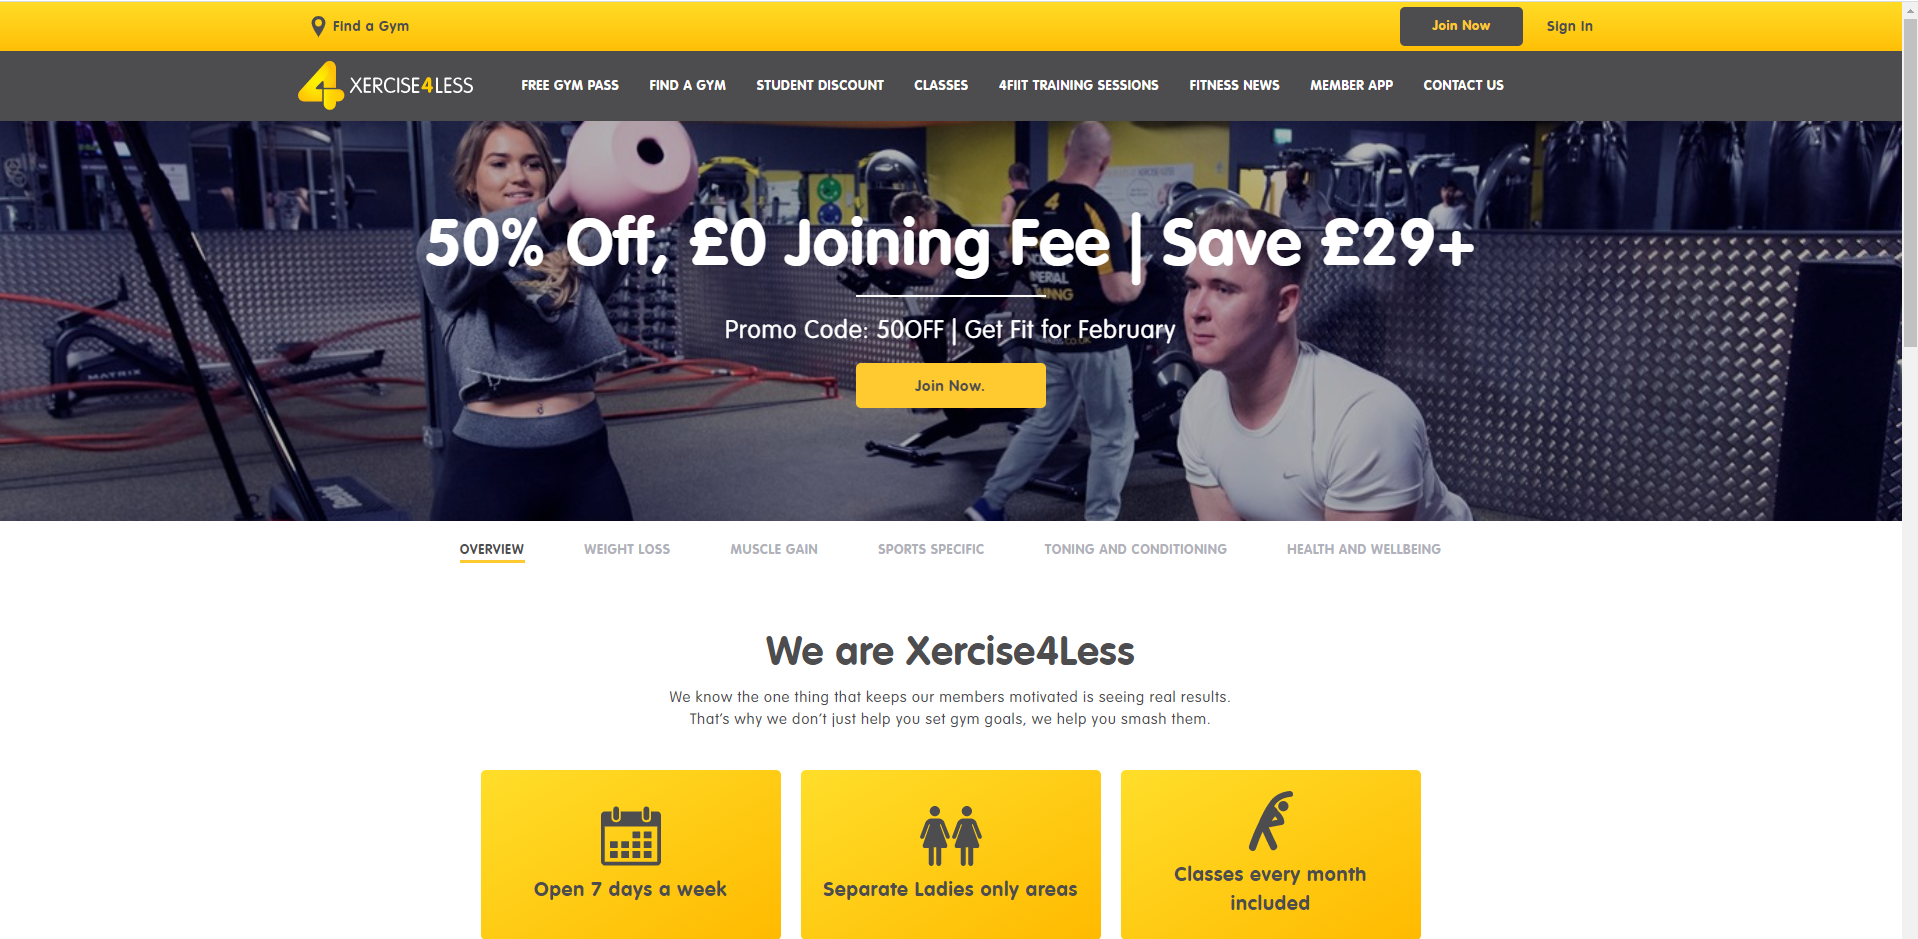
\includegraphics[width=0.7\linewidth]{img/gym/exercise4less-landing.png}\\
	 \textbf{Exercise4Less landing page}
\end{center}

\begin{center}
	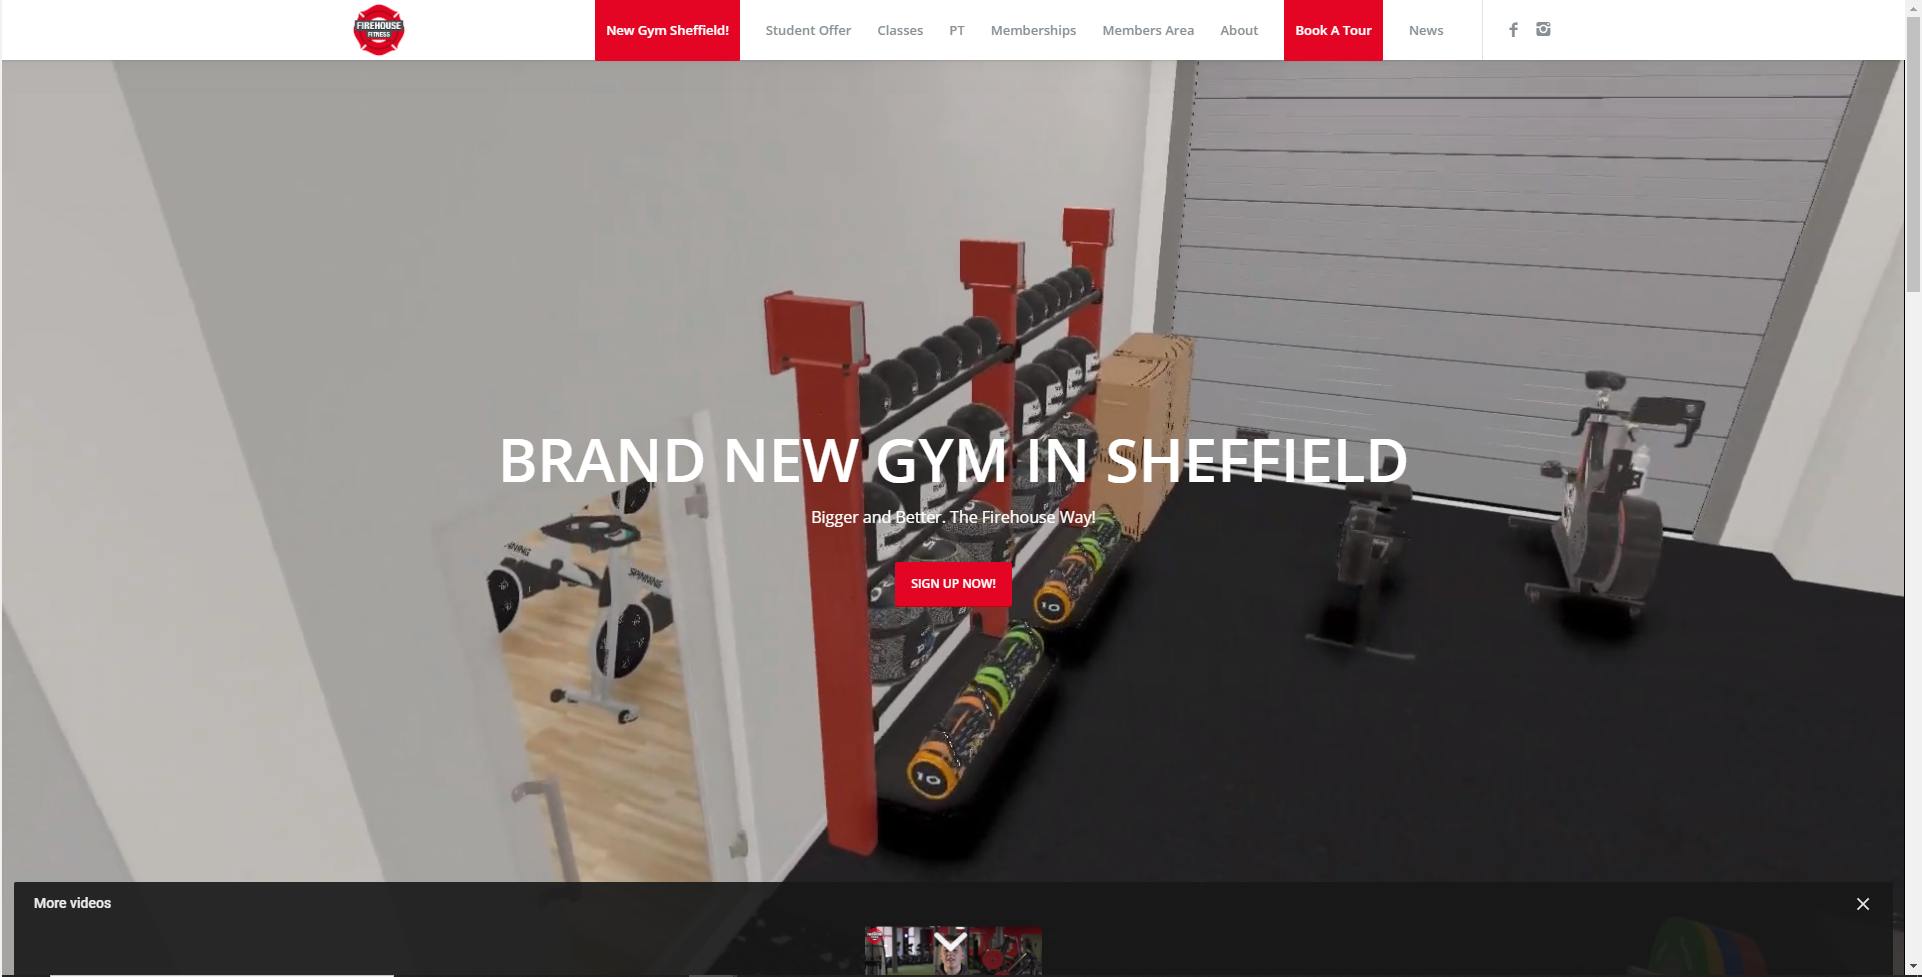
\includegraphics[width=0.7\linewidth]{img/gym/firehouse-landing.png}\\
	\textbf{Firehouse Fitness Gyms landing page}
\end{center}

\begin{itemize}
	\item All use large image in jumbotrop on landing page, here key info is displayed
	
	\item All feature clear membership or join buttons for joining the gyms
	
	\item Puregym, The gym and Exercise4Less all feature pricing as the first thing you see	
	
	\item Since these are chains, all (bar firehouse) include locators for specific location
	
	\item All use a minimalistic theme; lots of whites, big open spaces with large, bold text, light colours they convey a 'cool' mood
\end{itemize}




\section{Observations}

A good article to read is:

\begin{center}	
	https://www.templatemonster.com/blog/9-essential-sport-web-design-features/
\end{center}

Explains the relationship between colours and the mood they convey, the use of angles and polygons as seen in lots of the above examples; The Gym, Leisure Centre for example. Explains the use of proper positional items, including overlapping and simple fonts and the need for powerful imagery 

\subsection{Takeaway}

\begin{itemize}
	\item Use light colours, such as whites, blues and greens
	
	\item Make use of powerful imagery, such as on landing jumbotron, sports selection etc.
	
	\item Always show pricing and memberships on the landing page
	
	\item Include sections on wellbeing
	
	\item For admin, allow them to add new sports, view booking / reservations, change prices, add membership options, view members etc.
\end{itemize}


\subsection{Questions}

\begin{itemize}
	\item Who is the website meant for? will it include a centre locator like the gym or city council websites, or is it for a singular centre?
	
	\item Where will we get and licence the images from; all the websites make use of images, where will we get ours? If we use a free image site such as pexels how will we ensure images are relevant? If we licence images from existing centres how will we get permission?
	
	\item Will we have a database for different sports and activities, such that these can be extended, or will this be hard-coded? If the latter, how will reservations, memberships and booking interact with these entities?
	
	\item how will the interface for employees be considered; will this be integrated within the web application, or separate such as a desktop application?
	
	
	
	
\end{itemize}


\end{document}